% 2-var K-map for AB + A~B + ~AB = A + B
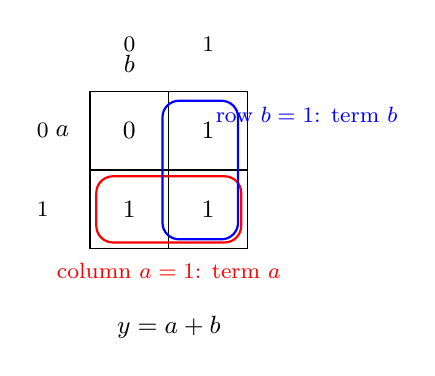
\begin{tikzpicture}[font=\small]
\draw[step=1] (0,0) grid (2,2);
\node at (-0.35,1.5) {$a$}; \node at (0.5,2.35) {$b$};
\node[font=\footnotesize] at (-0.6,1.5) {0}; \node[font=\footnotesize] at (-0.6,0.5) {1};
\node[font=\footnotesize] at (0.5,2.6) {0}; \node[font=\footnotesize] at (1.5,2.6) {1};
\node at (0.5,1.5) {0}; \node at (1.5,1.5) {1};
\node at (0.5,0.5) {1}; \node at (1.5,0.5) {1};
\draw[red, thick, rounded corners=6pt] (0.08,0.08) rectangle (1.92,0.92);
\node[red, font=\footnotesize] at (1.0,-0.28) {column $a=1$: term $a$};
\draw[blue, thick, rounded corners=6pt] (0.92,0.12) rectangle (1.88,1.88);
\node[blue, font=\footnotesize] at (2.75,1.7) {row $b=1$: term $b$};
\node at (1.0,-1.0) {$y = a + b$};
\end{tikzpicture}
